\documentclass[../main.tex]{subfiles}

\begin{document}

\chapter[Vulnerabilities in Primal Decomposition-based dMPC]{Vulnerabilities in \\Primal Decomposition-based \\distributed \\Model Predictive Control}\label{sec:primal_decomposition}
\epigraph{\centering All the world\\ is birthday cake,\\ so take a piece, \\but not too much.}
{\textit{It's All Too Much}\\\textsc{George Harrison}}

In this chapter we describe the optimization decomposition framework used in this work, founded on the definitions given in chapters~\ref{sec:decomposing_mpc} to~\ref{sec:anomalous} and giving insights of interpretation of each step.

Then we present the vulnerabilities of this framework illustrating with the consequences of some attacks.

\minitoc

\section{Primal decomposition-based \dmpc{}}\label{sec:decomposition_PD}

We start from the monolithic \mpc{} problem presented in~\eqref{eq:qp_standard_form}, which is reproduced here for the reader's convenience:
\begin{equation}
  \label{eq:qp_standard_form_reprise}
  \begin{aligned}
    \begin{matrix}
      \underset{\vec{U}[k]}{\mathrm{minimize}} &
      \frac{1}{2}\norm{\vec{U}[k]}^{2}_{H} + {\vec{f}[k]}^{T}\vec{U}[k] &\\
      \mathrm{subject~ to} &
\bar{\Gamma}\vec{U}[k]\preceq {\vec{U}}_{\text{max}}
    \end{matrix}
  \end{aligned}.
\end{equation}
As stated in~\ref{sec:qp_mpc}, the problem is an input constrained \qp{}, which is convex.

To decompose the problem with the optimization decomposition frameworks shown in~\S\ref{sec:decomp-fram} we assume the objective function of problem~\eqref{eq:qp_standard_form_reprise} to be decomposable into $M$ parts, which correspond to sub divisions of the initial system~\eqref{eq:large_scale_system_model} (corresponding sub-systems and sub-problems~\S\ref{sec:distributing_computation_units}).

Each sub-problem is given an index in set $\set{M}=\{1\mathbin{:}M\}$ and we can rewrite~\eqref{eq:qp_standard_form_reprise} as
\begin{equation}
  \label{eq:qp_standard_form_decomposable}
  \begin{aligned}
    \begin{matrix}
      \underset{\vec{U}_{1}[k],\dots, \vec{U}_{M}[k]}{\mathrm{minimize}} &
      \sum\limits_{i\in\set{M}}\left[\frac{1}{2}\norm{\vec{U}_{i}[k]}^{2}_{H_{i}} + {\vec{f}_{i}[k]}^{T}\vec{U}_{i}[k]\right]&\\
      \mathrm{subject~ to} & \sum\limits_{i\in\set{M}}\left[\bar{\Gamma}_{i}\vec{U}_{i}[k]\right] \preceq {\vec{U}}_{\text{max}}
    \end{matrix}
  \end{aligned},
\end{equation}
with local versions $\bar{\Gamma}_{i}$, $\vec{U}_{i}[k]$, $H_{i}$ and $\vec{f}_{i}[k]$ of variables presented in~\S\ref{sec:decomp-fram}.

Using the methodology in~\S\ref{sec:generalizing_decomposition} for coupling constraints, the primal decomposition divides the problem~\eqref{eq:qp_standard_form_decomposable} into a main problem~\eqref{eq:DOP_main} and local problems~\eqref{eq:DOP_local} based on the original primal problem~\eqref{eq:qp_standard_form_decomposable} and using interface variables $\thetaik,\forall i\in\set{M}$:
\begin{subequations}
  \begin{equation}
        J_{i}^{\star}(\thetaik)=
        \begin{matrix}
          \underset{\vec{U}_{i}[k]}{\mathrm{minimize}}&\obji=\frac{1}{2}\norm{\vec{U}_{i}[k]}^{2}_{H_{i}} + {\vec{f}_{i}[k]}^{T}\vec{U}_{i}[k]\\
          \mathrm{subject~ to} & \bar{\Gamma}_{i}\vec{U}_{i}[k] \preceq \thetaik:\lambdaik
      \end{matrix}
    \label{eq:DOP_local}
  \end{equation}

  \begin{equation}
    \begin{aligned}
      J^{\star}=
      \begin{matrix}
        \underset{\mpcvec{\theta}[i][k], \dots, \mpcvec{\theta}[M][k]}{\mathrm{minimize}} &\sum\limits_{i\in\set{M}} J^{\star}_i(\thetaik)\\
        \mathrm{subject~ to} &
          \begin{aligned}
            \quad \sum_{i\in\set{M}}\thetaik\preceq\vec{U}_{\max}\\
          \end{aligned}
      \end{matrix}
    \end{aligned},
    \label{eq:DOP_main}
  \end{equation}
\end{subequations}
where $\lambdaik,\forall i\in\set{M}$ are the dual variables of the problems, i.e. the lagrange multipliers associated with the constraints~\cite{BoydVandenberghe2004}.

Problem~\eqref{eq:DOP_main} is solved by updating the $\theta_{i}$ until convergence. The method chosen is the projected sub-gradient, which update is given by

\begin{equation}
  \label{eq:projectedSubgradient}
\vec{\theta}[k]\pplusone=\Proj^{\set{S}}(\vec{\theta}[k]\p-\rho\p\vec{g}[k]\p),
\end{equation}
where $\vec{\theta}[k]=[\vec{\theta}_{1}[k];\dots;\vec{\theta}_{M}[k]]$, ${\set{S} = \setbuild{\vec{\theta}[k]}{I_{c}^{M}\vec{\theta}[k]\preceq \vec{U}_{\max}}}$, being ${c=\card{\vec{U}_{\max}}}$, ${I_{c}^{M}=\kron{\1_{M}}{I_{c}}}$, $(p)$ is a given step in the iterative process and $\vec{g}\p[k]$ is a sub-gradient of the objective function of problem in~\eqref{eq:DOP_main} in step $p$.

From~\cite{BoydVandenberghe2004} and~\cite{BoydEtAl2015}, we can derive that the dual variables $\lambdaik$ of the local problems are sub-gradients of the main problem and can be used in~\eqref{eq:projectedSubgradient}, yielding

\begin{equation}
  \label{eq:projectedSubgradient}
\vec{\theta}[k]\pplusone=\Proj^{\set{S}}(\vec{\theta}[k]\p-\rho\p\vec{\lambda}[k]\p),
\end{equation}
with $\vec{\lambda}[k]=[\vec{\lambda}_{1}[k];\dots;\vec{\lambda}_{M}[k]]$.



\begin{description}
  \item[simple example to illustrate convergence]
  \item[Interpretation of variables] allocated resources and dissatisfaction index
\end{description}

\section[Anomalous behaviors and their consequences]{Anomalous behaviors and their consequences}\label{sec:vulnerabilities_PD}
% \epigraph{\centering So you tell me 'trust me' l can trust you\\ Just let me show you But I gotta work it out in a shadow of doubt 'Cause I don't know if I know you}
% {\textit{Lie}\\\textsc{Kevin Moore}}

\begin{remark}
  Observe that in this decomposition \textbf{``Liar'' agent attacks} as in \cite{VelardeEtAl2017b} cannot happen, since the input constraint is given by the coordinator.
\end{remark}

\begin{description}
  \item[Show examples of Attacks]
  \item[False data injection/communication corruption] \todo{show that since coordinator is oblivious to what happen inside each agent what matters is what it receives, no need to specify exactly the responsible part which generated attack}
\end{description}
but they will always reflect on the channel.
\begin{description}
  \item[Negotiation Stability] Show example and how cheating can destabilize negotiation
        \begin{enumerate}
          \item Analysis of eigenvalues of negotiation
        \end{enumerate}
  \item[Example of how attacker can drive negotiation to other points]
\end{description}
% \begin{figure}[h]
%   \centering
%   \begin{subfigure}{.45\textwidth}
%     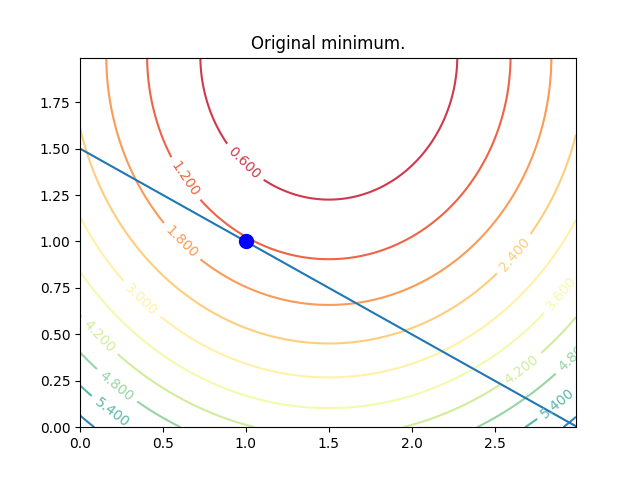
\includegraphics[width=\textwidth]{../img/original-minimum.png}
%     \caption{Original minimum.}
%     \label{fig:first}
%   \end{subfigure}
%   \hfill
%   \begin{subfigure}{0.45\textwidth}
%     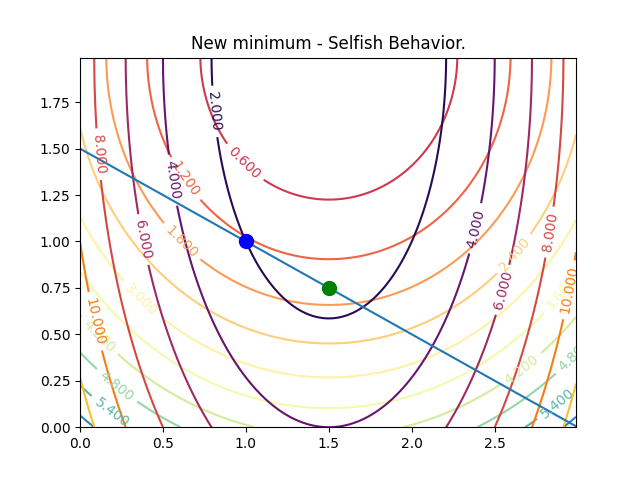
\includegraphics[width=\textwidth]{../img/new-minimum-selfish.png}
%     \caption{Minimum after non-conforming behavior.}
%     \label{fig:second}
%   \end{subfigure}
%   \caption{Effects of non-conforming behaviors on optimal value. \todo{Refaire les images}}
%   \label{fig:figures}
% \end{figure}

General discussion about ways to secure negotiation, here we discuss what
\begin{description}
  \item[Discussion about Methods]
  \item[Discussion about Detection and Isolation]
        \begin{description}
          \item[Learning methods] Use input labeled data to train detector
          \item[Analytical methods] Use model of the system and residuals
        \end{description}
  \item[Discussion about Recovery] Could show different cases
        \begin{description}
          \item[Active methods] Need detection
          \item[Passive methods] Robust control
        \end{description}
\end{description}


% \begin{figure}[h]
%   \centering
%   \begin{subfigure}{0.45\textwidth}
%     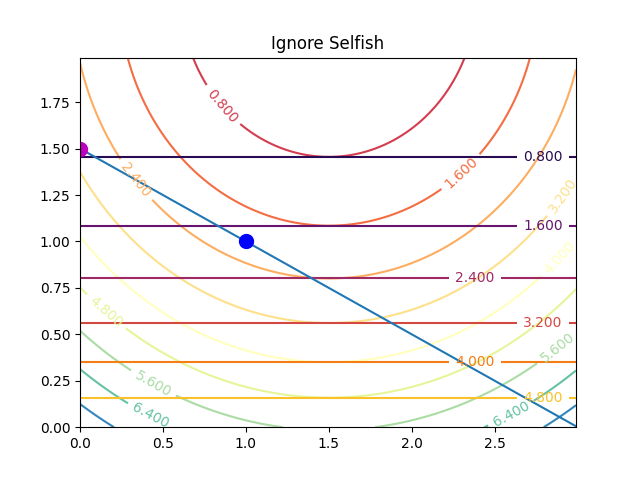
\includegraphics[width=\textwidth]{../img/ignoreX.png}
%     \caption{Optimal value after ignoring attacker.}
%     \label{fig:third}
%   \end{subfigure}
%   \hfill
%   \begin{subfigure}{0.45\textwidth}
%     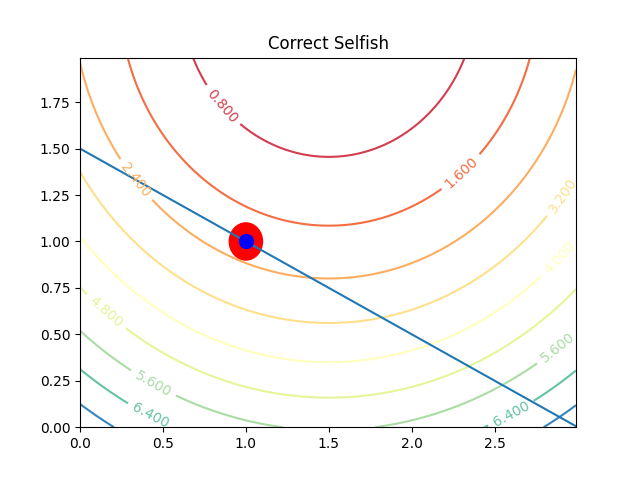
\includegraphics[width=\textwidth]{../img/correctX.png}
%     \caption{Optimal value after trying to recover original behavior.}
%     \label{fig:third}
%   \end{subfigure}

%   \caption{Recovering options.}
%   \label{fig:figures}
% \end{figure}


% Model 3R-2C \cite{GoudaEtAl2002}
% \begin{figure}[h]
%   \centering
%   \begin{circuitikz}[european]
%     \draw (0,0) node[tlground]{} to[isource, l=$P^{\text{heat}}$] ++(0,2) to[short, -*] ++(1.5,0) coordinate (a);

%     \draw (a) node[above]{$T^{\text{in}}$}  to[C=$C^{\text{air}}$] ++(0,-2) node[tlground]{};
%     \draw (0,-3) node[tlground]{} to[isource, l=$I^{\text{sol}}$] ++(0,2)
%     to[short, -*] ++(1.5,0) coordinate (b);
%     \draw (b) to[C=$C^{\text{walls}}$] ++(0,-2) node[tlground]{};

%     \draw (a) -- ++(2,0) coordinate (c) -- ++(0,-.5) to[R=$R^{\text{iw/ia}}$] ++(0,-2) -- ++(0,-.5) coordinate (d);

%     \draw (b) node[above]{$T^{\text{walls}}$} to[short,-*] (d);

%     \draw (c) --  ++(2.5,0) -- ++(0,-.5) to[R=$R^{\text{oa/ia}}$] ++(0,-2) -- ++(0,-.5) coordinate (e);

%     \draw (d) to[R=$R^{\text{ow/oa}}$] (e) to[battery,l=$T^{\text{out}}$] ++(0,-2) node[tlground]{};
%   \end{circuitikz}
%   \caption{Thermic Model 3R-2C of a room.}
%   \label{fig:3R2C_model}
% \end{figure}

The state-space model of each subsystem is given by:
\begin{equation}
  \begin{matrix}
    \label{eq:systems_cont}
    \dot{\vec{x}}_{i}(t)  &=&{A_{c}}_{i}\vec{x}_{i}(t) &+& {B_{c}}_{i}\vec{u}_{i}(t)\\
    \vec{y}_{i}(t)        &=&{C_{c}}_{i}\vec{x}_{i}(t) &&
  \end{matrix},
\end{equation}
where
\begin{equation}
  \label{eq:4}
  \begin{matrix}
    A_{\mathrm{c}_{i}}=\left[
      \begin{matrix}
        -\frac{1}{C^{\text{walls}}_{i}R^{\text{oa/ia}}_{i}}-\frac{1}{C^{\text{walls}}_{i}R^{\text{iw/ia}}_{i}}& \frac{1}{C^{\text{walls}}_{i}R^{\text{iw/ia}}_{i}}\\
        \frac{1}{C^{\text{air}}_{i}R^{\text{iw/ia}}_{i}} &-\frac{1}{C^{\text{air}}_{i}R^{\text{ow/oa}}o_{i}}-\frac{1}{C^{\text{air}}_{i}R^{\text{iw/ia}}_{i}}
      \end{matrix}\right]\\
    \begin{matrix}
      B_{\mathrm{c}_{i}}=\left[
        \begin{matrix}  \frac{10}{C^{\text{walls}}_{i}}& 0\end{matrix}
      \right]\T&C_{\mathrm{c}_{i}}=\left[\begin{matrix}1 & 0\end{matrix}\right]
    \end{matrix}
  \end{matrix}
\end{equation}
where ${\vec{x}_{i}=[{{x}_{A}}_{i}\T\ {{x}_{W}}_{i}\T]\T}$. ${x_A}_i$ and ${x_W}_i$ are the mean temperatures of the air and walls inside room~$i$. $\vec{u}_{i}$ is the input (the heating power)
for the corresponding room. The inputs are constraint by ${\sum_{i=1}^{4}\vec{u}_{i}(t)\preceq 4\mathrm{kW}}$.

\begin{table}[b]
  \centering
  \caption{Model Parameters}\label{tab:modelParamMeaning}
  \begin{tabular}[b]{cl}
    \toprule
    Symbol&Meaning\\
    \midrule
    $C^{\text{air}}_{i}$  &Heat Capacity of Inside Air\\
    $C^{\text{walls}}_{i}$ &Heat Capacity of External Walls\\
    $R^{\text{iw/ia}}_{i}$ &Resist. Between Inside Air and Inside Walls\\
    $R^{\text{ow/oa}}_{i}$ &Resist. Between Outside Air and Outside Walls\\
    $R^{\text{oa/ia}}_{i}$ &Resist. Between Inside and Out.\ Air (from windows)\\
    \bottomrule
  \end{tabular}
\end{table}

\begin{table}[b]
  \centering
  \caption{
    Parameters for each agent}\label{tab:modelParam}
  \begin{tabular}[t]{cccccc} \toprule
    Symbol& I & II & III & IV &Unit\\
    \midrule
    $C^{\text{walls}}$   &$5.4$&$4.9$&$4.7$&$4.7$ &$10^{4}\mathrm{J/K}$ \\
    $C^{\text{air}}$     &$7.5$ &$8.4 $&$8.2$ &$7.7$&$10^{4}\mathrm{J/K}$  \\
    $R^{\text{oa/ia}}$   &$5.2$&$4.6$&$4.9$&$5.4$&$10^{-3}\mathrm{K/W}$ \\
    $R^{\text{iw/ia}}$   &$2.3$&$2.4$&$2.3$&$2.9$&$10^{-4}\mathrm{K/W}$\\
    $R^{\text{ow/oa}}$   &$1.5$&$0.6$&$0.7$&$0.7$& $10^{-4}\mathrm{K/W}$ \\
    \bottomrule
  \end{tabular}
\end{table}

%\printbibliography

\end{document}
